\documentclass[12pt]{beamer}
\usetheme{Warsaw}
\usepackage[utf8]{inputenc}
\usepackage{amsmath}
\usepackage{amsfonts}
\usepackage{amssymb}
\usepackage{graphicx}
\usepackage[font=Times,timeinterval=1,timeduration=2.0,timedeath=0,fillcolorwarningsecond=white!60!yellow,timewarningfirst=50,timewarningsecond=80,resetatpages=2]{tdclock}
\usepackage{tabularx}
\usepackage{array}
\usepackage{multicol}
\usepackage{longtable}
\usepackage{xcolor}
\usepackage{textcomp, gensymb}
\usepackage{pgfplots}
\usepackage[makeroom]{cancel}

\graphicspath{ {./references/} }
\pgfplotsset{
	soldot/.style={color=black,only marks,mark=*},
	holdot/.style={color=black,fill=white,only marks,mark=*},
	compat=1.12
}
\newcolumntype{Y}{>{\centering\arraybackslash}X}
\makeatletter
\def\@listii{\leftmargin\leftmarginii
			  \topsep    2ex
			  \parsep    0\p@   \@plus\p@
			  \itemsep   \parsep}
\makeatother
\newcommand\at[2]{\left.#1\right|_{#2}}

\begin{document}
\begin{frame}
	\frametitle{Bellwork 11/15}
	\initclock

	\vfill
	\Large
	\[f(x)=\frac{\sin(x)}{x^2+x+1}\]
	\vfill
	\vfill
	Determine the local extrema of $f$ on $x\in[-2\text{, }2]$ with the first derivative test.
	\vfill
	\vfill
	\vfill
	\vfill
	\vfill
	\vfill

	\small
	\crono
	\resetcrono{\beamerbutton{reset}}
\end{frame}
\begin{frame}
	\frametitle{Bellwork 11/15 - Solution}

	Graph of $f'(x)$:
	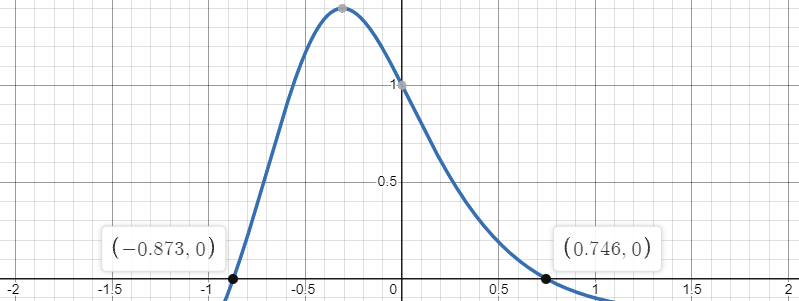
\includegraphics[scale=0.5]{exercise_1_solution_graph.png}
	\vfill
	Because $f'(x)$ changes signs at $x=-0.873\text{, }0.746$, local extrema are $f(-0.873)$ and $f(0.746)$.
	\[f(-0.873)=-0.862\text{; }f(0.746)=0.295\]
	\[\boxed{\text{Local Maximum: }0.295\text{; Local Minimum: }-0.862}\]
\end{frame}
\begin{frame}
	\frametitle{Exercise 1}

	\vfill
	\vfill
	\vfill
	\Large
	\[g(x)=x^2e^x\]
	\vfill
	Find the relative extrema of $g$ using the second derivative test.
	\vfill
	\vfill
	\vfill
\end{frame}
\begin{frame}
	\frametitle{Exercise 1 - Solution, Part 1}

	Find the critical points:
	\[g'(x)=2xe^x+x^2e^x=0\]
	\[\text{$e^x>0$ for all $x$}\implies (2x+x^2)\frac{\cancel{e^x}}{\cancel{e^x}}=\frac{0}{e^x}\implies x=-2\text{, }0\]
	Plug those $x$-values into the second derivative function:
	\[g''(x)=e^xx^2+4xe^x+2e^x=e^x(x^2+4x+2)\]
	\[g''(-2)=e^{-2}(4-8+2)=e^{-2}(-2)\text{; }g''(0)=2\]
\end{frame}
\begin{frame}
	\frametitle{Exercise 1 - Solution, Part 2}

	Because $g''(-2)<0$ and $g''(0)>0$, $g(-2)$ is the relative maximum while $g(0)$ represents the relative minimum of $g$.
	\[\boxed{\text{Local Maximum: }4e^{-2}\text{; Local Minimum: }0}\]
\end{frame}
\end{document}